\section{Reproducibility and Evidence Status}
\label{app:reproducibility}

\paragraph{Four evidence labels.}
Repository claims are tagged \texttt{verified}, \texttt{preregistered},
\texttt{planned}, or \texttt{literature-reported}.  Verified numeric claims
must resolve to committed endpoint CSVs and artifact manifests.
Preregistered indicates a fixed protocol without completed model outputs.
Planned rows are design commitments, not results.  Literature-reported rows
are protocol metadata from primary papers or official repositories and are
never merged with our measured table.

\paragraph{Verified run.}
The bounded run uses Pythia-70M revision
\texttt{a39f36b100fe} (the full hash is in the run manifest).  It selects six MLP
linear tensors, evaluates \VerifiedEvalTokens{} held-out next tokens, emits
all strategy artifacts, and stores natural/file bytes, SHA-256, round-trip
status, window NLL, 13-point paths, source/environment metadata, and process
completion evidence.  The numerical run predates source-file SHA capture for
its then-dirty working tree; this provenance limitation is disclosed rather
than reconstructed after the fact.

\paragraph{Scale suite.}
\path{scripts/run_large_scale_hessian_suite.py} expands a declarative
model/seed/rate/scope matrix.  It injects the repository's \texttt{src}
directory into the numerical subprocess, records config/job/source
fingerprints, and validates the exact selected tensor count and all artifact
hashes.  \texttt{RUNNING}, \texttt{FAILED}, stale partial directories, and
source drift are fail-closed.  Optional models require explicit selection.
The completed pilot has three \texttt{completed\_valid} jobs, 33 endpoint
files, 12 fixed-window comparisons, and 234 path rows.  Their numerical source
is \ScalePilotNumericalSourceSHA{}.  Each selected layer records the original
minimum eigenvalue relative to spectral scale, the float32 PSD floor, applied
diagonal shift, and final minimum eigenvalue; every downstream metric consumes
the same validated covariance.  The completed 2026-07-14 pilot used a
minimum-eigenvalue reduction with a zero initializer, so its positive minima
were conservatively reported as zero; those artifacts close the shift ledger
and final nonnegativity but do not claim an observed strictly positive stored
floor.  The revised, unexecuted runner reports the true minimum and separately
records the whitened-SVD fitting floor.  Both establish a usable PSD proxy,
not equality with the task Hessian.

\paragraph{Paper regeneration.}
Tables and numeric macros are generated by
\path{paper/results/build_verified_tables.py} and the fail-closed scale
aggregate by \path{paper/results/build_scaling_pilot.py}.  The latter verifies
suite/job/source fingerprints, checkpoint revisions, every physical file SHA,
Hessian decomposition, fixed windows, and Taylor paths before producing a
table or figure input.  Each plot script in
\texttt{paper/figures} reads committed CSVs and writes PDF, SVG, PNG, and a
manifest with input hashes.  No experimental point in this manuscript is
hand-entered into a plotting script.  The paper uses the official ICML 2026
style and can be compiled with Tectonic 0.16.9 using the commands documented in
\texttt{paper/README.md}.

\paragraph{External-method audit.}
The selected paper matrix records objective, updated state,
calibration/backward requirement, tensor and W/A/KV scope, payload fields,
official code status, and direct-comparison eligibility.  In particular,
LiftQuant block correction is a backward-assisted lane, while its optional
end-to-end correction is a global training lane.  A compatibility-patched
layer-0 smoke validates only one control path and artifact write; it supplies
no full-model PPL or same-byte result.  The repository retains a broader
59-row method registry.  Ten D-lane rows separately record multimodal/video
quantization, cache, sparse or structured attention, and sparse--low-rank
attention; they are scope-mismatched mechanism references rather than direct
LLM weight-PTQ controls.  The 27-row table below remains the primary-source
subset most directly tied to this paper's weight mechanisms and comparison
lanes.

\paragraph{Multimodal supplement.}
Video-DiT quantizers use temporal or attention-guided distillation
~\citep{feng2025qvdit,feng2025s2qvdit}; QuantSparse jointly optimizes
quantization and sparse attention~\citep{feng2025quantsparse}; and CacheQuant
jointly schedules diffusion caching and quantization
~\citep{liu2025cachequant}.  TeaCache, Sparse VideoGen, and Sparse-vDiT cover
timestep reuse and spatial/temporal sparse patterns
~\citep{liu2025teacache,xi2025sparsevideogen,chen2025sparsevdit}, while
VMonarch, MonarchRT, and RoPeSLR retain structured, dense-mixing, or low-rank
attention components~\citep{liang2026vmonarch,agarwal2026monarchrt,liu2026ropeslr}.
The repository supplement proposes a held-out gate among sink/global low rank,
local structure, dynamic sparse routes, and dense fallback, jointly accounted
with W/A PTQ, cache, and temporal reuse.  This is planned work: paper-reported
speedups are scope-specific and are never multiplied into a claimed stack.

\begin{table*}[t]
  \caption{Primary-source comparison audit.  Eligibility is determined by
  training dependence and exported state, not nominal bits alone.  Direct
  comparison additionally requires a matched checkpoint, tensor scope, data,
  and serializer.  Every external row is literature-reported.}
  \label{tab:lanes}
  \centering
  \scriptsize
\setlength{\tabcolsep}{3pt}
\begin{tabular}{@{}p{2.65cm}p{1.50cm}cp{4.05cm}p{4.10cm}c@{}}
\toprule
Method & Venue & Lane & Encoder process & Deployed state to charge & Exact file bytes? \\
\midrule
GPTQ~\citep{frantar2023gptq} & ICLR'23 & A1 & Activation Hessian proxy; no backward & Codes, scales, grouping/order metadata & No$^\dagger$ \\
SparseGPT~\citep{frantar2023sparsegpt} & ICML'23 & A1 & Second-order one-shot pruning & Values and explicit support/N:M layout & No$^\dagger$ \\
Wanda~\citep{sun2024wanda} & ICLR'24 & A1 & Weight--activation magnitude; no update & Values and explicit support/N:M layout & No$^\dagger$ \\
AWQ~\citep{lin2024awq} & MLSys'24 & A1 & Activation-aware scale/clipping search & Codes, scales and non-folded transforms & No$^\dagger$ \\
SpQR~\citep{dettmers2024spqr} & ICLR'24 & A1 & Second-order outlier separation & Bulk codes plus outlier values/indices & No$^\dagger$ \\
LQER~\citep{zhang2024lqer} & ICML'24 & A1 & Activation-scaled closed-form SVD & Base codec plus low-rank factors & No$^\dagger$ \\
QERA~\citep{zhang2025qera} & ICLR'25 & A1 & Closed-form reconstruction (PTQ row) & Base codec plus low-rank factors & No$^\dagger$ \\
EoRA~\citep{liu2024eora} & arXiv'24 & A1 & Eigenspace low-rank approximation & Compressed base plus low-rank factors & No$^\dagger$ \\
SLiM~\citep{mozaffari2025slim} & ICML'25 & A1 & One-shot quantization, 2:4 pruning, LR repair & Codes, 2:4 layout and low-rank factors & No$^\dagger$ \\
Harma et al.~\citep{harma2025effective} & ICLR'25 & A0 & Q/S order and non-orthogonality analysis & Sparse quantized values, scales and support & No$^\dagger$ \\
OBR~\citep{guo2026optimal} & ICLR'26 & A1 & Closed-form Hessian Q/S compensation & Folded sparse low-bit weights and layout & No$^\dagger$ \\
FOEM~\citep{zheng2026foem} & AAAI'26 & A1 & First-order proxy without backpropagation & Base-codec state after compensation & No$^\dagger$ \\
Radio~\citep{young2025radio} & ICML'25 & A1 & Post-training rate--distortion allocation & Codes plus allocation/decoder metadata & No$^\dagger$ \\
Q-Palette~\citep{lee2025qpalette} & NeurIPS'25 & A0/A1 & Data-free or calibrated mixed-scheme search & Codes, codebooks, scheme/fusion metadata & No$^\dagger$ \\
SRR~\citep{cho2026srr} & ICML'26 & A1 & Closed-form preserve/reconstruct rank split & Base codec plus both low-rank parts & No$^\dagger$ \\
SERQ~\citep{park2026serq} & ICLR'26 & A1 & Offline saliency decomposition/permutation & W/A codec, one LR matrix, permutation & No$^\dagger$ \\
ResComp~\citep{li2026rescomp} & ICLR'26 & A1 & Sequential compensation; no global tuning & Base codec plus any unabsorbed state & No$^\dagger$ \\
\midrule
SqueezeLLM~\citep{kim2024squeezellm} & ICML'24 & B & Loss-gradient-square/Fisher checkpoint & Indices, codebooks and sparse outliers & No$^\dagger$ \\
GuidedQuant~\citep{kim2025guidedquant} & ICML'25 & B & End-loss backward/Fisher blocks & Attached base-quantizer payload & No$^\dagger$ \\
Hessian ECSQ~\citep{choi2017towards} & ICLR'17 & B & Hessian-weighted entropy-constrained coding & Code stream, codebook/LUT and rate metadata & No$^\dagger$ \\
Optimal Formats~\citep{orr2025optimal} & arXiv'25 & B$^*$ & Variable-length formats; Fisher allocation & Streams, code tables and format allocation & No$^\dagger$ \\
SliderQuant~\citep{wang2026sliderquant} & ICLR'26 & B & Learned sliding-window scales and rank-4 repair & Codes plus any unmerged scale/low-rank state & No$^\dagger$ \\
YAQA~\citep{tseng2026yaqa} & ICML'26 & B & Full-model KL HVP/backward sketches & Quantizer payload; sketches are encoder-only & No$^\dagger$ \\
LiftQuant (block)~\citep{he2026liftquant} & ICML'26 & B & Block-output correction with backward passes & Lifted codes and projection/correction state & No$^\dagger$ \\
\midrule
LiftQuant (E2E)~\citep{he2026liftquant} & ICML'26 & C & Global causal-LM recovery & Learned lifted/projection/correction state & No$^\dagger$ \\
FPTQuant~\citep{vanbreugel2026fptquant} & ICML'26$^\ddagger$ & C & Locally and end-to-end learned transforms & Transformed codec and dynamic transform state & No$^\dagger$ \\
ProjQ~\citep{yu2026projq} & ICML'26 & C & Orthogonal Q/L projection plus adaptation & Base codec, adapter and projection state & No$^\dagger$ \\
\bottomrule
\multicolumn{6}{@{}p{16.3cm}@{}}{\footnotesize A0: data-free frozen compression; A1: calibrated/no-backward frozen compression; B: encoder-side backward/HVP without global recovery; C: learned or fine-tuned recovery. Optional QPEFT/PEFT results in QERA, SLiM, YAQA, and SRR are excluded from their A/B rows. $^*$Optimal Formats also contains a data-free format-analysis lane; B refers only to Fisher allocation. $^\dagger$The primary source reports bit width, sparsity, rank, logical memory, or runtime memory, but this audit found no complete deployable output-file byte enumeration including all codebooks, supports, factors, scales, headers, padding, and alignment. $^\ddagger$The official ICML 2026 listing and current arXiv metadata identify ICML 2026; an older OpenReview listing identifies ICLR 2026.} \\
\end{tabular}

\end{table*}

\begin{figure}[t]
  \centering
  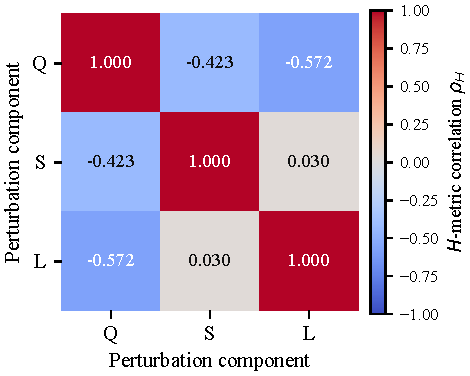
\includegraphics[width=\columnwidth]{figures/hessian_geometry.pdf}
  \caption{Signed activation-Gram correlations for the original conservative
  QSL endpoint, whose natural encoding is tail-padded to the Q+L final byte
  count.  S--L is near zero, while Q--S and Q--L are negative cancellation.
  Scope is one seed and six selected Pythia-70M MLP tensors.}
  \label{fig:geometry}
\end{figure}

\begin{table*}[t]
\centering
\caption{All native endpoints for the three scalability-smoke jobs. Rate and bits/parameter charge complete selected-tensor artifact files. The scopes and tokenizers differ, so rows must only be compared within each model block.}
\label{tab:scaling-pilot-all-endpoints}
\scriptsize
\resizebox{\textwidth}{!}{%
\begin{tabular}{llrrrrrrr}
\toprule
Model & Endpoint & Bytes & Rate & bits/sel. param & $\Delta$NLL & $\Delta$PPL & norm. $H$ & Repair (nnz/rank/dof) \\
\midrule
Pythia-70M & Q & 6,334,784 & 0.2517 & 4.028 & +0.3838 & +43.128 & 0.00961 & 0/0/0 \\
 & Q + global scale & 6,334,784 & 0.2517 & 4.028 & +0.3797 & +42.574 & 0.00946 & 0/0/12 \\
 & Q + block scale & 6,500,672 & 0.2583 & 4.133 & +0.2821 & +30.053 & 0.00597 & 0/0/98304 \\
 & Q+S & 6,520,898 & 0.2591 & 4.146 & +0.2532 & +26.562 & 0.00704 & 27276/0/0 \\
 & Q+S (OBS) & 6,520,898 & 0.2591 & 4.146 & +0.2273 & +23.533 & 0.00611 & 27276/0/27276 \\
 & Q+L & 6,497,344 & 0.2581 & 4.131 & +0.1963 & +19.994 & 0.00476 & 0/30/0 \\
 & Q+S+L strict & 6,497,344 & 0.2581 & 4.131 & +0.2060 & +21.094 & 0.00530 & 5248/16/0 \\
 & Q+S+L strict + scale & 6,497,344 & 0.2581 & 4.131 & +0.2017 & +20.603 & 0.00526 & 5248/16/30 \\
 & Q+S+L relaxed & 6,507,456 & 0.2585 & 4.137 & +0.2028 & +20.733 & 0.00475 & 6470/23/0 \\
 & Q+S (OBS)+L & 6,507,456 & 0.2585 & 4.137 & +0.1988 & +20.276 & 0.00476 & 6470/23/6470 \\
 & Q+S+L relaxed + scale & 6,507,456 & 0.2585 & 4.137 & +0.1993 & +20.333 & 0.00471 & 6470/23/30 \\
\addlinespace
OPT-125M & Q & 11,844,800 & 0.2510 & 4.016 & +0.1295 & +7.744 & 0.00585 & 0/0/0 \\
 & Q + global scale & 11,844,800 & 0.2510 & 4.016 & +0.1163 & +6.913 & 0.00576 & 0/0/10 \\
 & Q + block scale & 12,156,672 & 0.2576 & 4.122 & +0.0604 & +3.491 & 0.00337 & 0/0/175104 \\
 & Q+S & 12,195,064 & 0.2584 & 4.135 & +0.1080 & +6.390 & 0.00420 & 65560/0/0 \\
 & Q+S (OBS) & 12,195,064 & 0.2584 & 4.135 & +0.0999 & +5.884 & 0.00334 & 65560/0/65560 \\
 & Q+L & 12,158,976 & 0.2577 & 4.123 & +0.0735 & +4.272 & 0.00279 & 0/40/0 \\
 & Q+S+L strict & 12,158,976 & 0.2577 & 4.123 & +0.0828 & +4.835 & 0.00309 & 10528/23/0 \\
 & Q+S+L strict + scale & 12,158,976 & 0.2577 & 4.123 & +0.0744 & +4.328 & 0.00307 & 10528/23/30 \\
 & Q+S+L relaxed & 12,201,984 & 0.2586 & 4.138 & +0.0808 & +4.716 & 0.00305 & 13720/27/0 \\
 & Q+S (OBS)+L & 12,201,984 & 0.2586 & 4.138 & +0.0804 & +4.692 & 0.00302 & 13720/27/13720 \\
 & Q+S+L relaxed + scale & 12,201,984 & 0.2586 & 4.138 & +0.0727 & +4.224 & 0.00303 & 13720/27/30 \\
\addlinespace
Qwen3-0.6B & Q & 15,779,648 & 0.2508 & 4.013 & +0.1127 & +3.560 & 0.02295 & 0/0/0 \\
 & Q + global scale & 15,779,648 & 0.2508 & 4.013 & +0.1202 & +3.812 & 0.02204 & 0/0/10 \\
 & Q + block scale & 16,230,272 & 0.2580 & 4.128 & +0.0793 & +2.462 & 0.00662 & 0/0/245760 \\
 & Q+S & 16,254,218 & 0.2583 & 4.134 & +0.0420 & +1.280 & 0.00669 & 95090/0/0 \\
 & Q+S (OBS) & 16,254,218 & 0.2583 & 4.134 & +0.0260 & +0.786 & 0.00386 & 95090/0/95090 \\
 & Q+L & 16,196,352 & 0.2574 & 4.119 & +0.0226 & +0.683 & 0.00414 & 0/50/0 \\
 & Q+S+L strict & 16,196,352 & 0.2574 & 4.119 & +0.0303 & +0.918 & 0.00444 & 17440/30/0 \\
 & Q+S+L strict + scale & 16,196,352 & 0.2574 & 4.119 & +0.0299 & +0.905 & 0.00440 & 17440/30/30 \\
 & Q+S+L relaxed & 16,261,248 & 0.2584 & 4.135 & +0.0224 & +0.676 & 0.00415 & 25458/34/0 \\
 & Q+S (OBS)+L & 16,261,248 & 0.2584 & 4.135 & +0.0224 & +0.675 & 0.00419 & 25458/34/25458 \\
 & Q+S+L relaxed + scale & 16,261,248 & 0.2584 & 4.135 & +0.0219 & +0.660 & 0.00411 & 25458/34/30 \\
\bottomrule
\end{tabular}%
}
\end{table*}


\begin{figure*}[t]
  \centering
  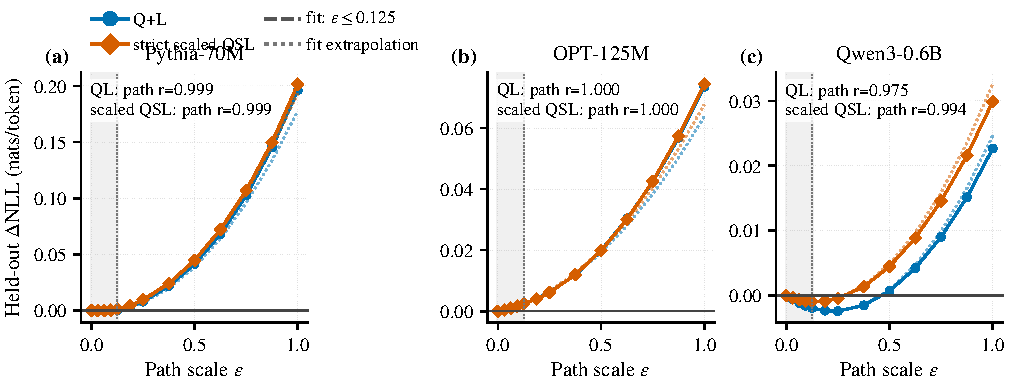
\includegraphics[width=0.99\textwidth]{figures/scaling_pilot_loss_paths.pdf}
  \caption{Thirteen-point one-dimensional interpolation probes for Q+L and
  strict component-scaled QSL in the three separate scalability-smoke jobs.
  Solid points are measured held-out NLL changes.  Dashed curves are fitted
  only on $\epsilon\le0.125$; lighter dotted continuations are extrapolations.
  The shaded region marks the fit interval, and each annotation is the
  path-specific proxy--NLL correlation over 13 points.  Panels use independent
  NLL scales and different tokenizers, so their magnitudes are not compared.
  These slices are not a global loss landscape or multi-seed evidence.}
  \label{fig:scaling-paths}
\end{figure*}
